\documentclass[12pt, letterpaper]{article}
\usepackage[utf8]{inputenc}
\usepackage{graphicx}
 
\title{Read Digits in Natural Scene Images using Convolutional Neural Networks }
\author{Ramesh Kumar(kumar.kumar@smail.inf.h-brs.de) \\ Roberto Cai Wu(roberto.cai@smail.inf.h-brs.de)}
\date{\today}
\begin{document}
\begin{titlepage}
\maketitle
\end{titlepage}

\section{Project Description}

	\begin{itemize}
		\item The project is about reading digits from the natural images with the help
		of convolutional neural networks(CNN).
			\item As Digit recognition is used in various applications such as postal mail sorting, bank check processing, form data entry, etcetera. 
\end{itemize}



%\textbf{Why Convolutional Neural Network}
%	\begin{itemize}
%		\item Since fast processing, accuracy and speed for these applications is important therefore, convolutional neural network is useful in this case.
		%\item Furthermore, according to state-of-the-art, it shows better performance as compare to other approaches\cite{Convolutional Neural Networks Applied to House Numbers Digit Classification}
	%\end{itemize}
%% Approach

\section{Approach}
The first part of this task consists of gathering data to train the network. We will use an already available dataset, Street View House Number (SVNH)\cite{Reading Digits in Natural Images
	with Unsupervised Feature Learning}. Images in this dataset come in various resolutions, colors, perspective, etcetera. In addition to this, we will create our own dataset to train and test on it. 
Images from dataset will be preprocessed before feeding to the network. Later on, post-processing will be needed in cases where an image contains multiple digits to get a final result by combining result of individual digit. 
\begin{itemize}
	\item Few possible approaches to solve this task are:
		\begin{itemize}
			\item Multiple hand-crafted features
			\item Template matching(might work on this also if time permits)
			\item Convolutional Neural Network(we use this)
		\end{itemize}
	\item Convolutional Neural Networks are used to extract features
	from the images and classify them. These networks are consists of different layers such as convolutional layers, pooling layers, and fully connected layers. Convolutional layer is first layer of the network that takes input as image and fully connected layer is final layer/output layer of the network that provides possible outcome based on input image.
	 %\item  \textbf{Challenges}
	%	\begin{itemize}
	%		\item Different Lighting conditions
	%		\item Design an appropriate network
	%		\item Different perspective view
	%		\item Blurred digits 
	%		\item Can be more when we start implementation
			
	%	\end{itemize}
	%\item For testing, we will test the images from live camera under various possible conditions such as hand-written digits, computerized-written digits, different lighting conditions, different font sizes, etcetera.
	\item Possible outcomes will be within 10 digit classes; one for each digit from label ``0'' to ``9'' and probability score of each outcome.
\end{itemize}

\section{Contribution}

\begin{itemize}
	\item Pre-processing using available dataset(Roberto Cai)
	\item Create the dataset and integrate with publicly available dataset (Ramesh Kumar)
	\item Create the Network(pair)
	\item Post-processing (Roberto Cai)
	\item Probability Score (Ramesh Kumar)
	\item Individual number combination in final result (Roberto Cai)
	\item Evaluation of approach (Ramesh Kumar)
	\item Documentation(pair)
\end{itemize}

\section{Sample images}
\begin{figure}[h]
\centering
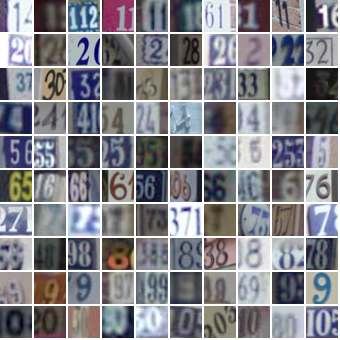
\includegraphics[width=0.5\textwidth]{dataset.png}
\caption{Dataset sample }
\end{figure}
\begin{figure}[h]
\centering
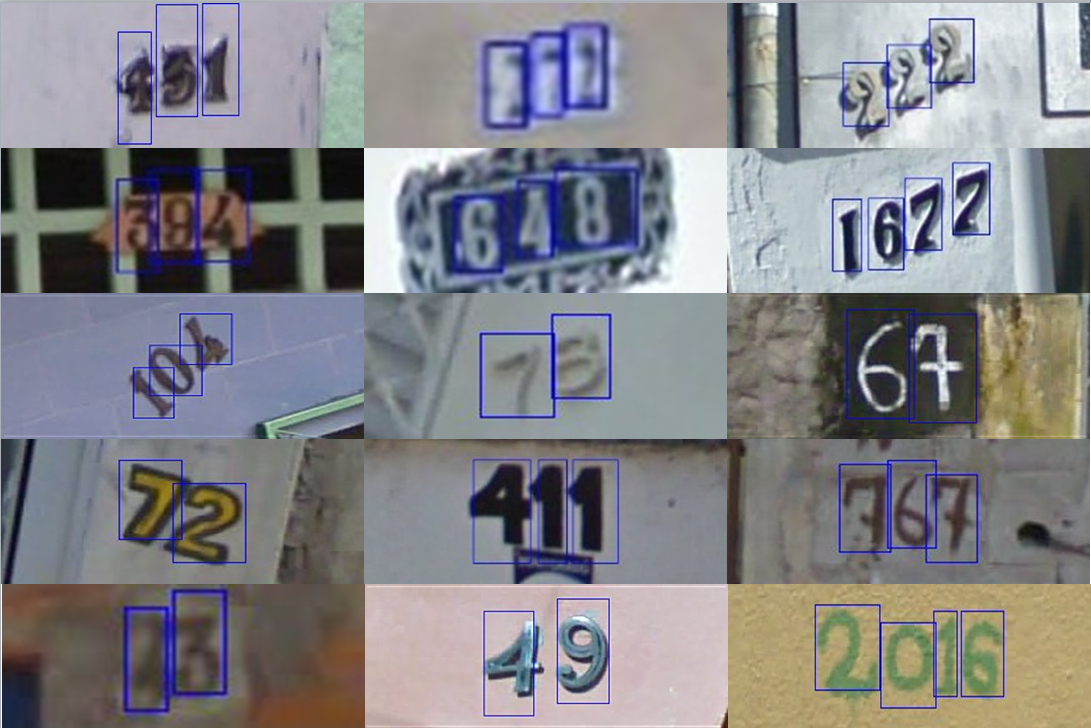
\includegraphics[width=0.5\textwidth]{example.png}
\caption{Expected result}
\end{figure}
\newpage
\begin{thebibliography}{9}
\bibitem{Convolutional Neural Networks Applied to House Numbers Digit Classification}
Pierre Sermanet, Soumith Chintala and Yann LeCun, "Convolutional Neural Networks Applied to
House Numbers Digit Classification", The Courant Institute of Mathematical Sciences - New York University 

\bibitem{Reading Digits in Natural Images
	with Unsupervised Feature Learning}

Yuval Netzer
, Tao Wang
, Adam Coates
, Alessandro Bissacco1
, Bo Wu
, Andrew Y. Ng, "Reading Digits in Natural Images
with Unsupervised Feature Learning", In NIPS Workshop on Deep
Learning and Unsupervised Feature Learning, 2011.

\end{thebibliography} 

\end{document}